% !TeX root=_main_.tex
% appendix1
% دستورات زیر باید در اولین فایل پیوست باشند. آنها را حذف نکنید!
\addtocontents{toc}
{
    \protect\renewcommand\protect\cftchappresnum{\appendixname~}%
    \protect\setlength{\cftchapnumwidth}{\mylenapp}
}%
    
\chapter{ساختار فایل PDF}\label{appendix:1}
\thispagestyle{empty}

در این پیوست به‌طور خلاصه ساختار کلی یک فایل \gls{PDF}
 را به‌عنوان یک ساختار فایل پیچیده بیان می‌کنیم. در فصل \ref{chapter1} اشاره کردیم که ویژگی‌های کامل قالب \gls{PDF}
  بسیار زیاد است. بیشتر این ویژگی‌ها، در حدود 70 درصد، در ارتباط با توضیح \glspl{DataObject} و ارتباط آنها بین بخش‌های مختلف یک فایل \gls{PDF}
   هست. تمرکز اصلی در این پیوست نیز بر روی ساختار \glspl{DataObject} خواهد بود. ما ساختار کلی \gls{PDF} را در دو بخش فیزیکی و منطقی بررسی خواهیم کرد.

فایل‌های \gls{PDF}
 در یک قالب متنی کدگذاری می‌شوند که ممکن است شامل \glspl{BinaryStream} مانند تصویر و غیره باشند. یک فایل \gls{PDF}
 ترکیبی از دست‌ِکم یک \gls{Body} است. یک \gls{Body} از سه بخش تشکیل شده است:  \gls{Object} (\lr{obj})، \gls{CrossReferenceTable} (\lr{xref})  و \lr{Trailer}. در ابتدای هر فایل یک سرآیند قرار می‌گیرد که با عبارت \lr{\%PDF} آغاز شده و در ادامه آن یک عدد که نگارش قالب \gls{PDF}
 را مشخص می‌کند، آمده است. ‏شکل \ref{appendix1_pdf_hello_world.png} یک فایل \gls{PDF}
  شامل متن  \lr{Hello Wrold} را که در یک ویراستار متنی باز شده است، نشان می‌دهد. در ادامه این ساختار را بررسی می‌کنیم.



\begin{figure}%[tbh!]%[ht]%[t!]
	\centering
	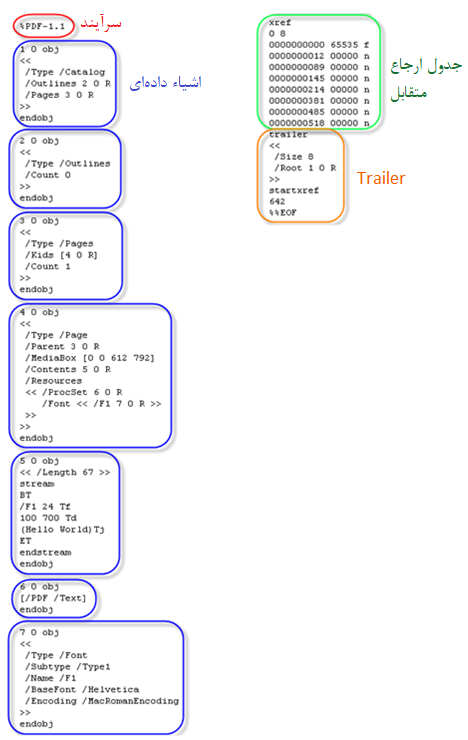
\includegraphics[width=0.8\textwidth, clip=true,  trim= 0 0 0 0]{appendix1/appendix1_pdf_hello_world.png}
	\caption[ یک فایل \gls*{PDF}  باز شده در یک ویراستار متنی شامل عبارت \lr{Hello World}]
	{
		یک فایل ساده \gls*{PDF} باز شده در یک ویراستار متنی شامل عبارت \lr{Hello Wrold}. چپ: سرآیند فایل و اشیای داده‌ای؛ اشیاء با مستطیل آبی (شماره‌های 1 تا 7) مشخص شده‌اند. راست: ادامه محتویات همان فایل، شامل جدول ارجاع متقابل و \lr{Trailer}.
	}
	\label{appendix1_pdf_hello_world.png}
	%\ref{appendix1_pdf_hello_world.png}
\end{figure}


\section{ساختار فیزیکی}\label{sec:physical_structure}
جزئیات ساختار فیزیکی بدنه فایل \gls*{PDF} به شرح زیر است:
\begin{itemize}
	\item{
		\textbf{اشیاء.}	
داده و فراداده در پرونده‌های \gls*{PDF}در یک واحد اولیه که شیء نامیده می‌شود سازماندهی می‌شوند. اشیا همگی قالب مشابهی دارند که در شکل \ref{appendix1_pdf_hello_world.png} مشخص است و همچنین یک ساختار بیرونی مشترک هم دارند. اولین خط یک شیء شناسه آن است که برای ارجاع‌های غیر مستقیم استفاده می‌شود. در ادامه عدد تولیدی آن است که اگر شی با یک نسخه جدیدتر بازنویسی شود، افزایش می‌یابد. سپس رشته 
\texttt{\lr{"obj"}}
 که شروع یک شیء را مشخص می‌کند آمده و پس از آن محتویات شیء قرار داده می‌شود. رشته 
 \texttt{\lr{"endobj"}}
 نیز پایان یافتن محدوده یک شیء را مشخص می‌کند.
	}

	\item{
		\textbf{جدول ارجاع متقابل.}	
	این جدول در بدنه \gls*{PDF} شامل آدرس نسبی اشیای مورد ارجاع قرار گرفته داخل یک فایل به صورت بایت می‌باشد. در شکل \ref{appendix1_pdf_hello_world.png} این جدول شامل 7 شیء با شناسه یک تا 7 و یک مکان نگهدارنده برای شناسه صفر است که به هیچ شیئی اشاره نمی‌کند.
	
	
	}

	\item{
		\textbf{\lr{Trailer}.}	
	 این قسمت از بدنه فایل \gls*{PDF} شامل یک \gls{Dictionary} از اطلاعات بدنه، مثل تعداد کل اشیای داخل فایل 
	 (\texttt{\lr{/size 8}})، شناسه و شماره ترتیبی شیء ریشه 
     (\texttt{\lr{/root 1 0 R}})
	 و غیره است. فرهنگ‌لغت بین نمادهای $ << $  و  $ >> $ قرار می‌گیرد. ادامه \lr{Trailer} شامل \lr{startxref} است که آدرس نسبی شروع جدول ارجاع متقابل در فایل را مشخص می‌کند. این فن اجازه می‌دهد تا بدنه از پایان با خواندن \lr{startxref} پویش شود، سپس به جدول ارجاع متقابل بازگشته و آن را نیز پویش می‌کند. بدین ترتیب تنها اشایی پویش می‌شوند که نیاز هستند. در شکل \ref{appendix1_pdf_hello_world.png} آدرس شروع جدول ارجاع متقابل که پس از \lr{startxref} در \lr{Trailer} آمده است برابر با 642 است. در صورتی که آدرس‌‌های بایت‌های این فایل بررسی شود، مشاهده خواهد شد که بایت 642ام شروع جدول ارجاع متقابل (کاراکتر \texttt{\lr{'x'}}) است. در پایانِ \lr{Trailer} نیز عبارت 
	 \texttt{\lr{\%\%EOF}}
	 قرار می‌گیرد که پایانِ فایل را مشخص می‌کند.
	
	}
\end{itemize}


ساختار جدول ارجاع متقابل و \lr{Trailer} به‌نسبت ساده و در فایل‌های گوناگون مشابه است، اما اشیای \gls{PDF}
 انواع محتلفی دارند. برای مثال شیء شماره 1 در شکل \ref{appendix1_pdf_hello_world.png}، حاوی یک ساختار فرهنگ ‌لغت است لذا بین نمادهای $ << $  و  $ >> $  واقع‌شده و حاوی کلیدهایی می‌شود که با کاراکتر $/$ شروع شده و در ادامه مقادیر آنها آمده است. مثلا مقدار 
\texttt{\lr{2 0 R}}
 یک ارجاع به شیئی در همین فایل با شناسه 2 و شماره ترتیبی 0 است. از آنجایی که یک فایل ممکن است خیلی بزرگ باشد؛ آدرس نسبی شیئی که به آن ارجاع داده شده است از طریق جدول ارجاع متقابل که یک جدول دسترسی تصادفی است، قابل دستیابی خواهد بود.
 
اشیای \gls{PDF}
 تنها محدود به فرهنگ لغت نمی‌شوند گرچه به‌نظر می‌آید که بیشتر آنها دست کم شامل یک فرهنگ لغت هستند. شیء شماره 5 در شکل \ref{appendix1_pdf_hello_world.png} برای نمونه، حاوی یک جریان دودویی است که بین واژه‌های کلیدی \lr{stream} و \lr{endstream} قرار گرفته است. تصاویر داخل \gls{PDF}
  نمونه‌ای از جریان‌های دودویی هستند که به این صورت می‌توانند ظاهر شوند. ‏شکل \ref{appendix1_pdf_stream_object.png}، یک شیء حاوی تصویر را نشان می‌دهد که در یک ویراستار متنی باز شده است.  شیء شماره 6 در شکل \ref{appendix1_pdf_hello_world.png} یک آرایه از کلید‌ها را شامل می‌شود. مقادیر آرایه می‌توانند انواع مختلفی داشته باشند که در هر صورت بین نمادهای $ [$  و $ ] $ قرار می‌گیرند و با کاراکتر فاصله از یکدیگر تمییز داده می‌شوند. به‌دلیل تنوع ذکر شده در ساختار اشیای \lr{PDF}، قواعد تعریف و ترکیب این اشیاء بیشترین بخش از توضیحات مشخصه‌های قالب فایل \gls{PDF}
  را تشکیل می‌دهند.


\begin{figure}%[tbh!]%[ht]%[t!]
	\centering
	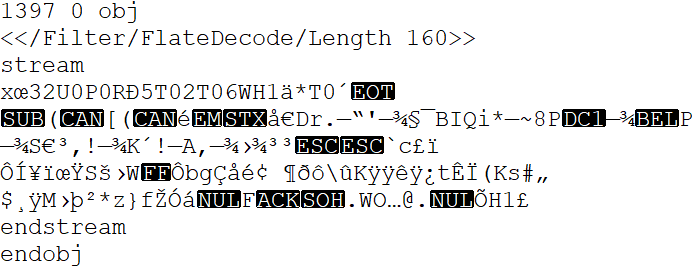
\includegraphics[width=0.9\textwidth, clip=true,  trim= 0 0 0 0]{appendix1/appendix1_pdf_stream_object.png}
	\caption[یک شیء \gls*{PDF} حاوی جریان دودویی]
	{
		یک شی \gls*{PDF}
		 حاوی یک تصویر. محتوای دودویی تصویر بین stream و endstream قرار گرفته است.
	}
	\label{appendix1_pdf_stream_object.png}
	%\ref{appendix1_pdf_stream_object.png}
\end{figure}

 
\section{ساختار منطقی}

آنچه در بخش \ref{sec:physical_structure} صحبت شد مربوط ساختار فیزیکی یک فایل \gls{PDF}
و نحوه قرار گرفتن اجزای فایل در کنار یکدیگر بود (مرتبط با گام پویش در هنگام اجرا). ساختار منطقی فایل \lr{PDF}، یعنی قواعد حاکم بر نحوه تفسیر و پردازش آنچه در یک فایل قرار دارد و ارتباط بین اجزا، یک ساختار سلسله مراتبی است (مرتبط با گام پرداخت در هنگام اجرا). شناسه شیء ریشه در Trailer مشخص می‌شود. به‌همین ترتیب شیء یا اشیای بعدی مورد نیاز در شیء ریشه معلوم می‌گردد. در فایل \gls{PDF}
شکل \ref{appendix1_pdf_hello_world.png} شیء شماره 1 ریشه است. اشیای شماره 2 و 3 داخل بدنه شیء 1 مورد دسترسی قرار می‌گیرند و در نهایت ترتیب نحوه دسترسی‌ها به‌صورت یک درخت قابل نمایش است که ساختار منطقی فایل را نشان می‌دهد. ‏شکل \ref{appendix1_pdf_logical_structure.png} ساختار منطقی فایل نشان داده شده در ‏شکل \ref{appendix1_pdf_hello_world.png} را نشان می‌دهد.


\begin{figure}%[tbh!]%[ht]%[t!]
	\centering
	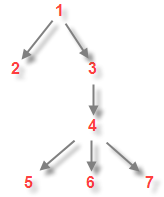
\includegraphics[clip=true,  trim= 0 0 0 0]{appendix1/appendix1_pdf_logical_structure.png}
	\caption[نمایش درختی ساختار منطقی فایل \gls*{PDF}]
	{
		ساختار منطقی فایل \gls*{PDF}
		 نشان داده شده در شکل \ref{appendix1_pdf_hello_world.png}. گره‌های درخت شناسه اشیاء در فایل \gls*{PDF}
		  و یال‌های آن معرف نحوه فراخوانی هر شی‌ء توسط شی‌ء دیگر هستند.
	}
	\label{appendix1_pdf_logical_structure.png}
	%\ref{appendix1_pdf_logical_structure.png}
\end{figure}



ساختار فیزیکی یک فایل \gls{PDF}
 را می‌توان بدون تغییر ساختار منطقی آن، به شکل دیگری تبدیل کرد. برای مثال در شکل \ref{appendix1_pdf_hello_world.png} اشیاء به‌ترتیب صعودی شناسه خود در فایل ظاهر شده بودند. می‌‌شود ترتیب قرارگرفتن اشیاء را به‌صورت نزولی در آورد. در این صورت جدول ارجاع متقابل بایستی بروزرسانی شود؛ زیرا، هر شی در در مکان متفاوتی نسبت به قبل قرار گرفته است. اما این پدیده تأثیری بر ساختار منطقی ندارد. ساختار منطقی کماکان همان ساختار ‏شکل \ref{appendix1_pdf_logical_structure.png} و نتیجه اجرا نیز با فایل قبلی یکسان خواهد بود. جدول ارجاع متقابل برای حالتی که اشیاء به صورت نزولی در فایل ظاهر شده باشند، در ‏شکل \ref{appendix1_xref_updated.png} نشان داده شده است.



\begin{figure}%[tbh!]%[ht]%[t!]
	\centering
	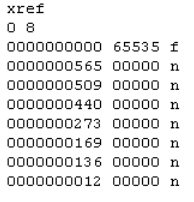
\includegraphics[clip=true,  trim= 0 0 0 0]{appendix1/appendix1_xref_updated.png}
	\caption[جدول ارجاع متقابل بروزرسانی شده یک فایل \gls*{PDF}]
	{
		جدول ارجاع متقابل بروزرسانی شده در حالتی که اشیاء به ترتیب نزولی شناسه خود در فایل \gls*{PDF}
		 ظاهر شده‌اند.
	}
	\label{appendix1_xref_updated.png}
	%\ref{appendix1_xref_updated.png}
\end{figure}



به‌طور کلی اشیاء \gls{PDF}
می‌توانند در مکان‌های تصادفی داخل یک فایل \gls{PDF}
 ظاهر شوند بدون اینکه تأثیر بر پرداخت فایل داشته باشند. برای فایل ساده ‏شکل \ref{appendix1_pdf_hello_world.png} تنها با تعویض ترتیب ظاهر شدن اشیاء می‌توان تعداد 5040 (برابر با !7) فایل با ساختار فیزیکی متفاوت داشت. این درحالی است که تغییر ترتیب قرارگیری اشیا تنها یک روش برای جابه‌جایی ساختار فیزیکی فایل \gls{PDF}
  است و روش‌های دیگری مثل تغییر محل قرارگیری جدول ارجاع متقابل نیز وجود دارد. بنابراین رابطه بین ساختار منطقی و فیزیکی فایل \gls{PDF}
  به صورت یک به چند است.

\section{بروزرسانی فایل PDF}

دیدیم که چگونه ساختار منطقی فایل \gls{PDF}
مستقل از ساختار فیزیکی آن شکل می‌گیرد. بروزرسانی فایل \gls{PDF}
 بر همین مبنا است. فایل‌های \gls{PDF}
 می‌توانند به‌صورت \gls{Incremental} بروزرسانی شوند. بدین ترتیب که اگر نویسنده فایل \gls{PDF}
  بخواهد اطلاعات داخل شیء شماره 7 را بروزرسانی کند، یک بدنه جدید آغاز می‌کند. سپس محتوای شیء جدید را داخل آن نوشته، عدد تولیدی (عدد بعد از شناسه شیء) را یک واحد نسبت به عدد تولیدی شیء قدیم افزایش داده و برای شی جدید می‌نویسد. در  انتها نیز یک جدول ارجاع متقابل را که به شیء جدید اشاره می‌نماید، تولید کرده و بدنه جدید را به سند قبلی الصاق می‌کند.













